%% bare_conf.tex
%% V1.4b
%% 2015/08/26
%% by Michael Shell
%% See:
%% http://www.michaelshell.org/
%% for current contact information.
%%
%% This is a skeleton file demonstrating the use of IEEEtran.cls
%% (requires IEEEtran.cls version 1.8b or later) with an IEEE
%% conference paper.
%%
%% Support sites:
%% http://www.michaelshell.org/tex/ieeetran/
%% http://www.ctan.org/pkg/ieeetran
%% and
%% http://www.ieee.org/

%%*************************************************************************
%% Legal Notice:
%% This code is offered as-is without any warranty either expressed or
%% implied; without even the implied warranty of MERCHANTABILITY or
%% FITNESS FOR A PARTICULAR PURPOSE! 
%% User assumes all risk.
%% In no event shall the IEEE or any contributor to this code be liable for
%% any damages or losses, including, but not limited to, incidental,
%% consequential, or any other damages, resulting from the use or misuse
%% of any information contained here.
%%
%% All comments are the opinions of their respective authors and are not
%% necessarily endorsed by the IEEE.
%%
%% This work is distributed under the LaTeX Project Public License (LPPL)
%% ( http://www.latex-project.org/ ) version 1.3, and may be freely used,
%% distributed and modified. A copy of the LPPL, version 1.3, is included
%% in the base LaTeX documentation of all distributions of LaTeX released
%% 2003/12/01 or later.
%% Retain all contribution notices and credits.
%% ** Modified files should be clearly indicated as such, including  **
%% ** renaming them and changing author support contact information. **
%%*************************************************************************


% *** Authors should verify (and, if needed, correct) their LaTeX system  ***
% *** with the testflow diagnostic prior to trusting their LaTeX platform ***
% *** with production work. The IEEE's font choices and paper sizes can   ***
% *** trigger bugs that do not appear when using other class files.       ***                          ***
% The testflow support page is at:
% http://www.michaelshell.org/tex/testflow/



\documentclass[conference]{IEEEtran}
% Some Computer Society conferences also require the compsoc mode option,
% but others use the standard conference format.
%
% If IEEEtran.cls has not been installed into the LaTeX system files,
% manually specify the path to it like:
% \documentclass[conference]{../sty/IEEEtran}





% Some very useful LaTeX packages include:
% (uncomment the ones you want to load)


% *** MISC UTILITY PACKAGES ***
%
%\usepackage{ifpdf}
% Heiko Oberdiek's ifpdf.sty is very useful if you need conditional
% compilation based on whether the output is pdf or dvi.
% usage:
% \ifpdf
%   % pdf code
% \else
%   % dvi code
% \fi
% The latest version of ifpdf.sty can be obtained from:
% http://www.ctan.org/pkg/ifpdf
% Also, note that IEEEtran.cls V1.7 and later provides a builtin
% \ifCLASSINFOpdf conditional that works the same way.
% When switching from latex to pdflatex and vice-versa, the compiler may
% have to be run twice to clear warning/error messages.






% *** CITATION PACKAGES ***
%
%\usepackage{cite}
% cite.sty was written by Donald Arseneau
% V1.6 and later of IEEEtran pre-defines the format of the cite.sty package
% \cite{} output to follow that of the IEEE. Loading the cite package will
% result in citation numbers being automatically sorted and properly
% "compressed/ranged". e.g., [1], [9], [2], [7], [5], [6] without using
% cite.sty will become [1], [2], [5]--[7], [9] using cite.sty. cite.sty's
% \cite will automatically add leading space, if needed. Use cite.sty's
% noadjust option (cite.sty V3.8 and later) if you want to turn this off
% such as if a citation ever needs to be enclosed in parenthesis.
% cite.sty is already installed on most LaTeX systems. Be sure and use
% version 5.0 (2009-03-20) and later if using hyperref.sty.
% The latest version can be obtained at:
% http://www.ctan.org/pkg/cite
% The documentation is contained in the cite.sty file itself.






% *** GRAPHICS RELATED PACKAGES ***
%
\ifCLASSINFOpdf
  \usepackage[pdftex]{graphicx}
  % declare the path(s) where your graphic files are
  % \graphicspath{{../pdf/}{../jpeg/}}
  % and their extensions so you won't have to specify these with
  % every instance of \includegraphics
  \DeclareGraphicsExtensions{.pdf,.jpeg,.png,.jpg}
\else
  % or other class option (dvipsone, dvipdf, if not using dvips). graphicx
  % will default to the driver specified in the system graphics.cfg if no
  % driver is specified.
  % \usepackage[dvips]{graphicx}
  % declare the path(s) where your graphic files are
  % \graphicspath{{../eps/}}
  % and their extensions so you won't have to specify these with
  % every instance of \includegraphics
  % \DeclareGraphicsExtensions{.eps}
\fi
% graphicx was written by David Carlisle and Sebastian Rahtz. It is
% required if you want graphics, photos, etc. graphicx.sty is already
% installed on most LaTeX systems. The latest version and documentation
% can be obtained at: 
% http://www.ctan.org/pkg/graphicx
% Another good source of documentation is "Using Imported Graphics in
% LaTeX2e" by Keith Reckdahl which can be found at:
% http://www.ctan.org/pkg/epslatex
%
% latex, and pdflatex in dvi mode, support graphics in encapsulated
% postscript (.eps) format. pdflatex in pdf mode supports graphics
% in .pdf, .jpeg, .png and .mps (metapost) formats. Users should ensure
% that all non-photo figures use a vector format (.eps, .pdf, .mps) and
% not a bitmapped formats (.jpeg, .png). The IEEE frowns on bitmapped formats
% which can result in "jaggedy"/blurry rendering of lines and letters as
% well as large increases in file sizes.
%
% You can find documentation about the pdfTeX application at:
% http://www.tug.org/applications/pdftex





% *** MATH PACKAGES ***
%
\usepackage{amsmath}
\usepackage{amsfonts}
% A popular package from the American Mathematical Society that provides
% many useful and powerful commands for dealing with mathematics.
%
% Note that the amsmath package sets \interdisplaylinepenalty to 10000
% thus preventing page breaks from occurring within multiline equations. Use:
%\interdisplaylinepenalty=2500
% after loading amsmath to restore such page breaks as IEEEtran.cls normally
% does. amsmath.sty is already installed on most LaTeX systems. The latest
% version and documentation can be obtained at:
% http://www.ctan.org/pkg/amsmath





% *** SPECIALIZED LIST PACKAGES ***
%
%\usepackage{algorithmic}
% algorithmic.sty was written by Peter Williams and Rogerio Brito.
% This package provides an algorithmic environment fo describing algorithms.
% You can use the algorithmic environment in-text or within a figure
% environment to provide for a floating algorithm. Do NOT use the algorithm
% floating environment provided by algorithm.sty (by the same authors) or
% algorithm2e.sty (by Christophe Fiorio) as the IEEE does not use dedicated
% algorithm float types and packages that provide these will not provide
% correct IEEE style captions. The latest version and documentation of
% algorithmic.sty can be obtained at:
% http://www.ctan.org/pkg/algorithms
% Also of interest may be the (relatively newer and more customizable)
% algorithmicx.sty package by Szasz Janos:
% http://www.ctan.org/pkg/algorithmicx




% *** ALIGNMENT PACKAGES ***
%
%\usepackage{array}
% Frank Mittelbach's and David Carlisle's array.sty patches and improves
% the standard LaTeX2e array and tabular environments to provide better
% appearance and additional user controls. As the default LaTeX2e table
% generation code is lacking to the point of almost being broken with
% respect to the quality of the end results, all users are strongly
% advised to use an enhanced (at the very least that provided by array.sty)
% set of table tools. array.sty is already installed on most systems. The
% latest version and documentation can be obtained at:
% http://www.ctan.org/pkg/array


% IEEEtran contains the IEEEeqnarray family of commands that can be used to
% generate multiline equations as well as matrices, tables, etc., of high
% quality.




% *** SUBFIGURE PACKAGES ***
\ifCLASSOPTIONcompsoc
  \usepackage[caption=false,font=normalsize,labelfont=sf,textfont=sf]{subfig}
\else
  \usepackage[caption=false,font=footnotesize]{subfig}
\fi
% subfig.sty, written by Steven Douglas Cochran, is the modern replacement
% for subfigure.sty, the latter of which is no longer maintained and is
% incompatible with some LaTeX packages including fixltx2e. However,
% subfig.sty requires and automatically loads Axel Sommerfeldt's caption.sty
% which will override IEEEtran.cls' handling of captions and this will result
% in non-IEEE style figure/table captions. To prevent this problem, be sure
% and invoke subfig.sty's "caption=false" package option (available since
% subfig.sty version 1.3, 2005/06/28) as this is will preserve IEEEtran.cls
% handling of captions.
% Note that the Computer Society format requires a larger sans serif font
% than the serif footnote size font used in traditional IEEE formatting
% and thus the need to invoke different subfig.sty package options depending
% on whether compsoc mode has been enabled.
%
% The latest version and documentation of subfig.sty can be obtained at:
% http://www.ctan.org/pkg/subfig




% *** FLOAT PACKAGES ***
%
%\usepackage{fixltx2e}
% fixltx2e, the successor to the earlier fix2col.sty, was written by
% Frank Mittelbach and David Carlisle. This package corrects a few problems
% in the LaTeX2e kernel, the most notable of which is that in current
% LaTeX2e releases, the ordering of single and double column floats is not
% guaranteed to be preserved. Thus, an unpatched LaTeX2e can allow a
% single column figure to be placed prior to an earlier double column
% figure.
% Be aware that LaTeX2e kernels dated 2015 and later have fixltx2e.sty's
% corrections already built into the system in which case a warning will
% be issued if an attempt is made to load fixltx2e.sty as it is no longer
% needed.
% The latest version and documentation can be found at:
% http://www.ctan.org/pkg/fixltx2e


%\usepackage{stfloats}
% stfloats.sty was written by Sigitas Tolusis. This package gives LaTeX2e
% the ability to do double column floats at the bottom of the page as well
% as the top. (e.g., "\begin{figure*}[!b]" is not normally possible in
% LaTeX2e). It also provides a command:
%\fnbelowfloat
% to enable the placement of footnotes below bottom floats (the standard
% LaTeX2e kernel puts them above bottom floats). This is an invasive package
% which rewrites many portions of the LaTeX2e float routines. It may not work
% with other packages that modify the LaTeX2e float routines. The latest
% version and documentation can be obtained at:
% http://www.ctan.org/pkg/stfloats
% Do not use the stfloats baselinefloat ability as the IEEE does not allow
% \baselineskip to stretch. Authors submitting work to the IEEE should note
% that the IEEE rarely uses double column equations and that authors should try
% to avoid such use. Do not be tempted to use the cuted.sty or midfloat.sty
% packages (also by Sigitas Tolusis) as the IEEE does not format its papers in
% such ways.
% Do not attempt to use stfloats with fixltx2e as they are incompatible.
% Instead, use Morten Hogholm'a dblfloatfix which combines the features
% of both fixltx2e and stfloats:
%
% \usepackage{dblfloatfix}
% The latest version can be found at:
% http://www.ctan.org/pkg/dblfloatfix




% *** PDF, URL AND HYPERLINK PACKAGES ***
%
\usepackage{url}
% url.sty was written by Donald Arseneau. It provides better support for
% handling and breaking URLs. url.sty is already installed on most LaTeX
% systems. The latest version and documentation can be obtained at:
% http://www.ctan.org/pkg/url
% Basically, \url{my_url_here}.




% *** Do not adjust lengths that control margins, column widths, etc. ***
% *** Do not use packages that alter fonts (such as pslatex).         ***
% There should be no need to do such things with IEEEtran.cls V1.6 and later.
% (Unless specifically asked to do so by the journal or conference you plan
% to submit to, of course. )

\usepackage{multirow}
\usepackage[binary-units=true,detect-weight=true]{siunitx}

% correct bad hyphenation here
\hyphenation{ImageNet}

\DeclareMathOperator*{\argmin}{argmin}
\DeclareMathOperator{\sign}{sign}
\DeclareMathOperator{\popcount}{popcount}
\DeclareMathOperator{\bn}{BatchNormalize}

\usepackage{etoolbox}
\makeatletter
\patchcmd{\@makecaption}
  {\scshape}
  {}
  {}
  {}
\makeatother

\begin{document}
\title{XNOR Networks for Embedded Systems}

\author{\IEEEauthorblockN{Andrei Cramariuc}
\IEEEauthorblockA{Semester Project, Autumn 2016\\
Integrated Systems Laboratory\\
crandrei@student.ethz.ch}
\and
\IEEEauthorblockA{Supervisor}
\IEEEauthorblockN{Prof. Luca Benini}
\IEEEauthorblockA{Co-supervisors}
\IEEEauthorblockN{Lukas Cavigelli\\
Renzo Andri}}

\maketitle

\begin{abstract}
Convolutional neural networks (CNNs) have risen to be the most commonly used classifiers nowadays in domains such as image and audio processing, for their ability to model complex data. One of the disadvantages of CNNs is the huge computational complexity and the large amount of memory that is required for both training and inference, where most of the workload is usually offloaded onto power-hungry and large Graphical Processing Units (GPUs). On the other hand there exist many applications on low-power embedded systems that would benefit from using state-of-the-art classifiers, but are currently limited by the high energy and computational demands of CNNs. This project explores the possibility of using XNOR networks which are CNN that have been trained to only use binary weights and activations, thus reducing the amount of required memory and speeding up computation significantly. The disadvantage of this quantization is that XNOR networks have on average a 10\% lower accuracy. The aim of this project will be to implement, train and test an XNOR network on a microcontroller.
\end{abstract}

\section{Introduction}
Convolutional neural networks have significantly advanced the limits of machine learning in a wide variety of tasks in the domains of image and audio processing. CNNs are currently considered state-of-the-art classifiers when it comes to problems such as object recognition \cite{best1}, image segmentation \cite{best2} and speech recognition \cite{best3}. Many modern technologies such as self driving cars, facial detection algorithms and image tagging algorithms rely heavily on CNNs.

Today, due to the high amount of computational power required to train and run CNNs, they are almost exclusively used in conjunction with one or more GPUs \cite{best1}. GPUs offer a considerable speed up by calculating in parallel a large amount required computations, but at the cost of a significant increase in energy consumption. Using GPUs also adds the need for dedicated hardware which increases the amount of required space and the cost of production.

Large amounts of memory are required because CNNs have very many floating-point parameters, sometimes even hundreds of millions. For example, a typical CNN structure for image classification such as AlexNet has \SI{61}{M} parameters that need to be stored and a forward pass requires a total of 1.5 billion high precision operations per image \cite{alexnet}. As a result it is a challenge to run CNNs on low-power devices with limited amounts of computational power, memory and storage. Having a state-of-the-art classifier running on embedded systems would be beneficial in many situations in which processing the data off-chip is not possible or transmitting the data would be more costly than processing it locally. Examples of possible applications include the concept of Internet of Things (IoT), which is gaining popularity due to the rising number of sensors being integrated into our everyday lives, through things such as smart phones, health bracelets and household appliances \cite{iot}. Another benefit is the possibility of locally analysing data on existing platforms which satisfies many privacy concerns. Other applications include satellites where data transmission is complicated or mobile robots that would need to be able to operate completely independently \cite{robots}.

As there is significant interest in enabling the usage of CNNs on embedded platforms different approaches have been proposed. One of these approaches is to simplify the neural network design, by using shallow networks that in theory can approximate any decision boundary but in practice are difficult to train \cite{deep}. Another possible simplification is using more compact layers, which can be done for example by replacing the fully connected layers at the top of a CNN with global average pooling \cite{compact1} or replacing convolutional filters with smaller ones \cite{compact2}. Another approach to simplify neural networks is compressing them by pruning unused parameters, removing unused connections and quantizing existing weights \cite{prune}, \cite{quantize}. A more drastic approach to quantization is binarizing all the parameters in the network during training and inference \cite{binary}.

This project aims to implement and test the method proposed in Rastegari \textit{et al.} \cite{xnor}. They binarize both the parameters and the activations of the network, to produce what they call XNOR networks. This binarization greatly reduces the required amount of memory and computational power but introduces an equally big quantization error. Parameters can now be stored using only one bit instead of a 32-bit floating-point and multiplications can be done using bitwise operation, addition and subtraction. Using only binary values it is also possible to perform several multiplications at the same time by storing multiple binary parameters in the same variable. This project aims to explore how this method can be applied to other networks than the one tested in Rastegari \textit{et al.} \cite{xnor} and also to test the applicability of the method in practice on a microcontroller.

\section{Related works}

\subsection{XNOR neural networks}
Rastegari \textit{et al.} explore the option of binarizing both the weights and the activations of a CNN so that all the values are represented by either $1$ or $-1$ \cite{xnor}. In practice these values can be represented by only one bit instead of the 32 bits which are required to represent a floating-point value in a standard CNN layer.

Given a floating-point filter $\mathbf{W}\in\mathbb{R}^{h\times w\times c}$ of height $h$, width $w$ and with $c$ input channels, the aim is to estimate $\mathbf{W}$ with a binary filter $\mathbf{B}\in\{+1,-1\}^{h\times w\times c}$ using a scaling factor $\alpha \in \mathbb{R}^{+}$ so that 
\begin{equation}
\mathbf{W}\approx\alpha\mathbf{B}
\label{eq:approx}
\end{equation}
To solve $\mathbf{B}$ and $\alpha$ we have an optimization problem that can be written as
\begin{equation}
\argmin_{\mathbf{B}, \alpha}\ \lvert\lvert\mathbf{W} - \alpha\mathbf{B}\rvert\rvert^2
\end{equation}
for which the solution is
\begin{align}
\mathbf{B} &= \sign(\mathbf{W}) \\
\alpha &= \frac{1}{n}\lvert\lvert\mathbf{W}\rvert\rvert_{l1}
\label{eq:alpha}
\end{align}
where $n=h\cdot w\cdot c$ is the number of elements in $\mathbf{W}$ \cite{xnor}. Therefore the optimal binary filter is $\mathbf{W}$ thresholded at zero and the optimal scaling factor is the average of the absolute values of $\mathbf{W}$. Also the fully connected layers of a CNN can be binarized using this method. This is because a fully connected layer can be written as a set of filters where there are as many filters as there are neurons on the fully connected layer and all the filters are equal in size to the previous layer. Therefore the above rule is sufficient in binarizing the majority of the parameters of a CNN.

\begin{figure}[!t]
\centering
\subfloat[Standard]{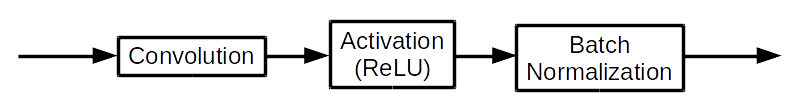
\includegraphics[width=\columnwidth]{nn1}%
\label{fig:structure-normal}}
\hfill
\subfloat[XNOR]{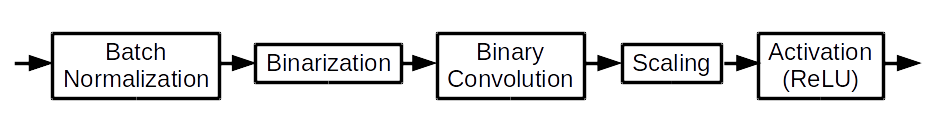
\includegraphics[width=\columnwidth]{nn2}%
\label{fig:structure-xnor}}
\caption{The basic blocks in the structure of standard CNNs and XNOR networks.}
\end{figure}

Binarizing the activations $\mathbf{A}\in\mathbb{R}$ is done through adding a threshholding layer equivalent to $\sign(\mathbf{A})$ and slightly reorganizing the network structure to compensate for the error caused by the quantization. A block from which a standard CNN is formed is described in Figure \ref{fig:structure-normal}. When binarizing the activations the batch normalization is moved before the binarization. Here the batch normalization layer normalizes the input and applies an affine transform learned during the training phase. The batch normalization layer can be described as
\begin{equation}
\bn(\mathbf{A}) = \frac{\mathbf{A}-\mu}{\sigma}\cdot\gamma + \beta
\label{eq:bn-matrix}
\end{equation}
where $\mu$ is the mean of the batch, $\sigma$ is the standard deviation of the batch, and $\gamma$ and $\beta$ are the parameters of the affine transform learned during training. Situating the batch normalization layer before the binarization makes it so the network tcan learn the optimal scaling factor and threshold for the following binarization layer.

After binarizing both the activations and the weights of the network, the convolution operation can be done using only bitwise operations, addition and subtraction. This approach avoids the use of multiplication which on many embedded systems is a costly operation without dedicated hardware support. When a Floating-Point Unit (FPU) is not available, multiplication operations between floating-point values are emulated in software using fixed-point operations. Emulated fixed-point operations are slower because they require multiple basic operations, as opposed to a FPU which can perform most operations in a single instruction cycle.

The training of the network still has to be done using full-precision weights, because the gradient update would otherwise be too small to influence the weights. During training the full precision network is binarized and the direction of the gradient is calculated. The stochastic gradient descent algorithm then updates the weights of the full-precision network based on the direction of the gradient. The activations are binarized similarly during training and run time.

Rastegari \textit{et al.} tested XNOR networks on AlexNet trained on the ImageNet classification task \cite{xnor}. The ImageNet dataset consists of 10 million hand labeled images from over \mbox{10 000} categories. The network was trained on a subset of ImageNet containing 1.2 million images from 1000 categories \cite{imagenet}. Nowadays the best results that have been obtained on ImageNet have a mean average precision of 66\% \cite{imagenet-res}. Using full-precision weight and activations the resulting accuracy for the network trained by Rastegari \textit{et al.} was 56.6\%. Binarizing the weights did not affect the accuracy, but also binarizing the activations resulted in an accuracy of 44.2\%. \cite{xnor}

\subsection{Audio event classification}

\begin{figure}[!t]
\centering
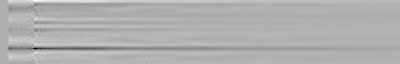
\includegraphics[width=\columnwidth]{mfcc}
\caption{The MFCCs of a guitar string as a 64$\times$400px image}
\label{fig:mfcc}
\end{figure}

\begin{figure*}[!t]
\centering
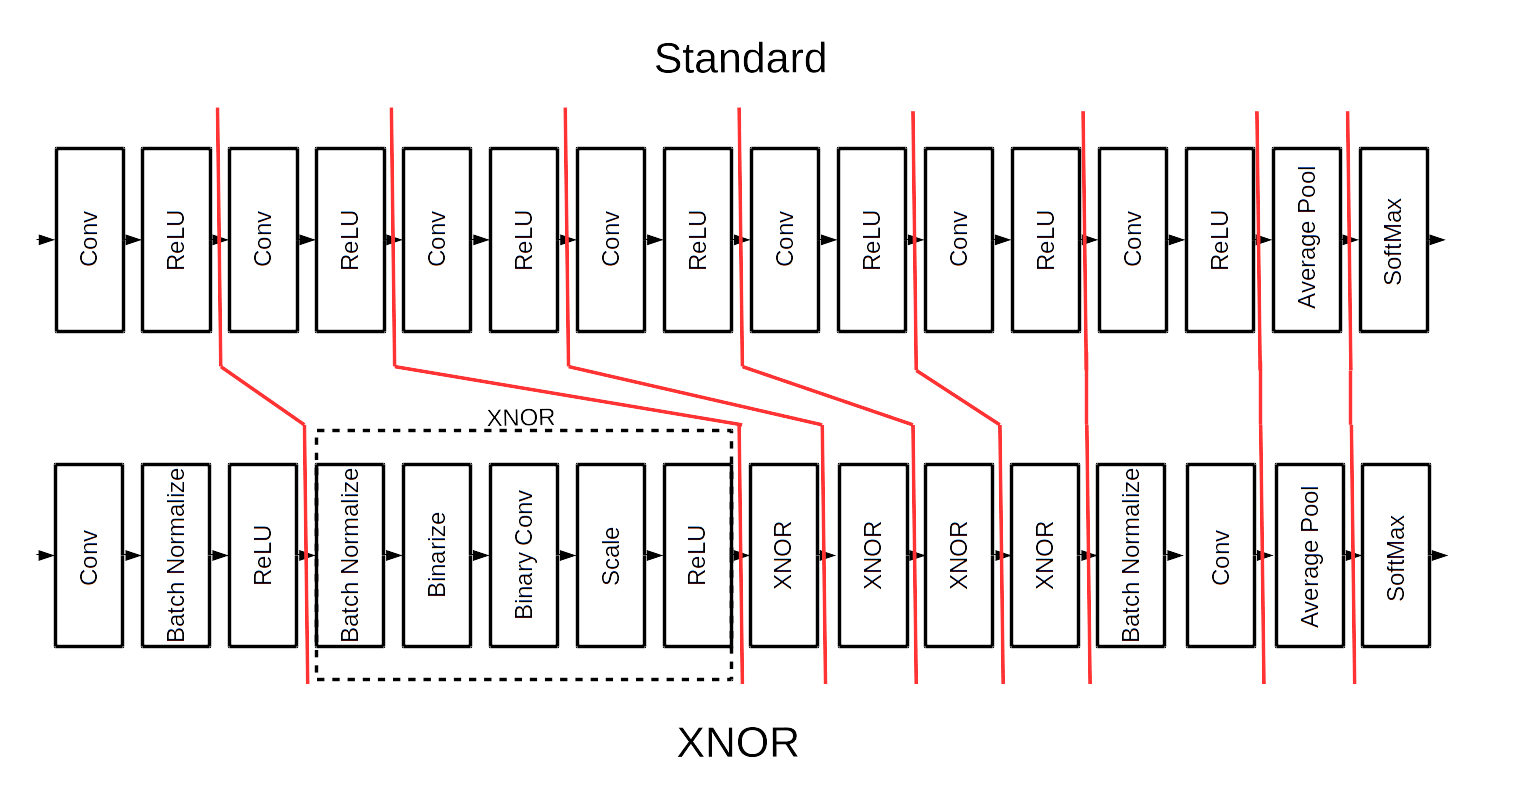
\includegraphics[width=\textwidth]{nn-full}
\caption{At the top is the CNN structure proposed by Meyer \textit{et al.} and at the bottom is the modified XNOR network structure \cite{lukas}.}
\label{fig:nn-full}
\end{figure*}

To test XNOR networks this project focused on binarizing and implementing the network published by Meyer \textit{et al.} \cite{lukas}. This network was trained classifying audio events into 28 classes including: cat, laughter, helicopter, engine, footstep, bird, violin and dog sounds. The dataset with which the network was trained consists of a total of 5223 audio samples at \SI{16}{\kilo\hertz} and with a varying length of 1 to 20 seconds and a total duration of 768 minutes.

The preprocessing was done using the Mel-frequency cepstral coefficients (MFCCs). The MFCCs of a signal are obtained by taking the Fourier transform of a signal and mapping the logarithms of the powers of the spectrum onto the mel scale. Afterwards the MFCCs are the amplitudes obtained from the discrete cosine transform of the list of mel logarithmic powers. The one-dimensional audio signal is transformed into a two-dimensional image by windowing the audio signal and taking the 64-point MFCCs of each window and placing them as consecutive columns in an image. Figure \ref{fig:mfcc} shows what the sound of a swinging guitar string looks like. In total the image contains 400 windows each with 400 samples and where consecutive windows overlap 75\%. Each window therefore represents 2.5 seconds of audio at \SI{16}{\kilo\hertz}. MFCCs are used because they compactly represent the frequencies in sounds similarly to how humans perceive them. MFCCs have been successfully used in modelling both speech and music \cite{mfcc}.

\begin{table}[!t]
\renewcommand{\arraystretch}{1.3}
\caption{Network structure described by  Meyer \textit{et al.} \cite{lukas}.}
\label{table:param-normal}
\centering
\begin{tabular}{|l|r|r|}
\multicolumn{1}{c}{\bfseries Layer} & \multicolumn{1}{c}{\bfseries Parameters} & \multicolumn{1}{c}{\bfseries Memory}\\
\hline
conv 3$\times$3, 32 & \SI{320}{} & \SI{1}{\kilo\byte} \\
\hline
conv 3$\times$3, 64 & \SI{18}{k} & \SI{72}{\kilo\byte} \\
\hline
conv 3$\times$3, 128 & \SI{72}{k} & \SI{288}{\kilo\byte} \\
\hline
conv 3$\times$3, 128 & \SI{144}{k} & \SI{576}{\kilo\byte} \\
\hline
conv 3$\times$3, 128 & \SI{144}{k} & \SI{576}{\kilo\byte} \\
\hline
conv 1$\times$1, 128 & \SI{16}{k} & \SI{64}{\kilo\byte} \\
\hline
conv 1$\times$1, 28 & \SI{3.5}{k} & \SI{14}{\kilo\byte} \\
\hline
\multicolumn{1}{c}{\bfseries Total:} & \multicolumn{1}{r}{\bfseries \SI{395}{k}} & \multicolumn{1}{r}{\bfseries \SI{1.6}{\mega\byte}}\\
\end{tabular}
\end{table}

\begin{table}[!t]
\renewcommand{\arraystretch}{1.3}
\caption{Number of parameters for each feature map in the network.}
\label{table:feature}
\centering
\begin{tabular}{|c|r|r|r|}
\multicolumn{1}{c}{\multirow{2}{*}{\bfseries Conv layer}} & \multicolumn{1}{c}{\bfseries Feature map} & \multicolumn{1}{c}{\bfseries Memory} &  \multicolumn{1}{c}{\bfseries Memory}\\

\multicolumn{1}{c}{\quad} & \multicolumn{1}{c}{\bfseries parameters} & \multicolumn{1}{c}{\bfseries (full-precision)} &  \multicolumn{1}{c}{\bfseries (XNOR)}\\

\hline
1 & \SI{25}{k} & \SI{100}{\kilo\byte} & \SI{100}{\kilo\byte}\\
\hline
2 & \SI{800}{k} & \SI{3200}{\kilo\byte} & \SI{100}{\kilo\byte} \\
\hline
3 & \SI{400}{k} & \SI{1600}{\kilo\byte} & \SI{50}{\kilo\byte} \\
\hline
4 & \SI{800}{k} & \SI{3200}{\kilo\byte} & \SI{100}{\kilo\byte} \\
\hline
5 & \SI{200}{k} & \SI{800}{\kilo\byte} & \SI{25}{\kilo\byte}\\
\hline
6 & \SI{200}{k} & \SI{800}{\kilo\byte} & \SI{25}{\kilo\byte}\\
\hline
7 & \SI{200}{k} & \SI{800}{\kilo\byte} & - \\
\hline
output & \SI{44}{k} & \SI{176}{\kilo\byte} & - \\
\hline
\end{tabular}
\end{table}

The CNN structure proposed by Meyer \textit{et al.} has in total 7 convolutional layers which are listed in Table \ref{table:param-normal} \cite{lukas}. In Table \ref{table:param-normal} each row in the first column represents the size of the convolutional filter and the number of filters. The second column is the number of parameters for each layer and the third column is the amount of memory needed when using floating-point units. The structure of the network is in Figure \ref{fig:nn-full}. The network has already been compressed by replacing the fully connected layers at the top with smaller convolutional layers and a global average pooling layer. The total number of parameters is \SI{395}{k} and the memory required to store them is \SI{1.6}{\mega\byte} when using floating-points. The size of the feature map that each convolutional layer takes as input is in Table \ref{table:feature} and the total amount of required intermediary storage is the sum of the two largest consecutive feature maps, which is \SI{1200}{k} parameters. When using 32-bit floating-point values the network would require about \SI{1.6}{\mega\byte} of memory for weights and \SI{4.7}{\mega\byte} for feature maps, which is a total of \SI{6.2}{\mega\byte}. The full-precision network achieved a top-1 classification accuracy of 86\% and a top-5 classification accuracy of 100\% \cite{lukas}.


\section{Implementation}

\subsection{Network structure}
\label{sec:net}

\begin{table}[!t]
\renewcommand{\arraystretch}{1.3}
\caption{Number of parameters of the equivalent XNOR network for the CNN described by Meyer \textit{et al.} \cite{lukas}.}
\label{table:param-xnor}
\centering
\begin{tabular}{|c|r|r|r|}
\multicolumn{1}{c}{\bfseries Conv layer} & \multicolumn{1}{c}{\bfseries Binary} & \multicolumn{1}{c}{\bfseries Floating-point} & \multicolumn{1}{c}{\bfseries Memory}\\
\hline
1 & - & \SI{448}{} & \SI{2}{\kilo\byte} \\
\hline
2 & \SI{18}{k} & \SI{256}{} & \SI{3}{\kilo\byte} \\
\hline
3 & \SI{72}{k} & \SI{512}{} & \SI{11}{\kilo\byte} \\
\hline
4 & \SI{144}{k} & \SI{768}{} & \SI{21}{\kilo\byte} \\
\hline
5 & \SI{144}{k} & \SI{768}{} & \SI{21}{\kilo\byte} \\
\hline
6 & \SI{16}{k} & \SI{768}{} & \SI{5}{\kilo\byte} \\
\hline
7 & - & \SI{4}{k} & \SI{16}{\kilo\byte}\\
\hline
\multicolumn{1}{c}{\bfseries Total:} & \multicolumn{1}{r}{\bfseries \SI{394}{k}} & \multicolumn{1}{r}{\bfseries \SI{7.4}{k}} & \multicolumn{1}{r}{\bfseries \SI{79}{\kilo\byte}}\\
\end{tabular}
\end{table}

\begin{figure}[!t]
\centering
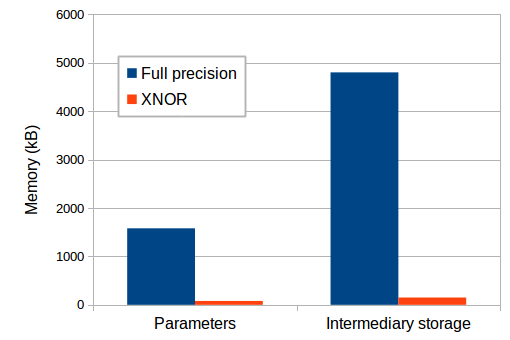
\includegraphics[width=0.75\columnwidth]{mem}
\caption{Diagram of how the data is organized in the feature map of the XNOR network.}
\label{fig:mem}
\end{figure}

The network structure proposed by Meyer \textit{et al.} was modified according to the changes proposed by Rastegari \textit{et al.} \cite{xnor}, \cite{lukas}. The weights for the first and last convolutional layers and their activations were not binarized, because they caused a too significant loss in accuracy \cite{xnor}. Not binarizing these layers has only a minor impact on the reduction in complexity and required memory, due to the fact that the first and last layer are the smallest in the network as can be seen from Table \ref{table:param-normal}. The full-precision intermediary storage required by the last layer can be ignored in practice since the last layer can be combined with the previous layer and the resulting output can be directly accumulated into the global average pooling layer. Therefore the maximum amount of required intermediary storage for the XNOR network is \SI{150}{\kilo\byte}.

As opposed to what was suggested in \cite{xnor} the activation layers were left in the binarized version of the network, because it was empirically determined that keeping them increased the final accuracy. A batch normalization layer was added between the first convolutional layer and proceeding ReLU layer. The activation layer proceeding the last convolutional layer was removed and a batch normalization layer was added in front of the convolutional layer. The intermediary five convolutional layers and their activation layers were replaced with a batch normalization, a binzarization, a binary convolution, a scaling and a ReLU layer. The final structure of the network is in Figure \ref{fig:nn-full} and can be compared with the original network structure in Figure \ref{fig:nn-full}.

The non binary parameters still remaining in the XNOR network structure are the bias and scaling factor of each binary convolutional filter, the batch normalization parameters and the full-precision first and last convolutional layers. Table \ref{table:param-xnor} contains the total number of full precision and binary parameters, which require a total of \SI{79}{\kilo\byte}. The ratio between the number of full-precision parameters and binary parameters remains less than 2\%. The total amount of require memory for a XNOR net is \SI{230}{\kilo\byte} which is 28 times less than for the original network. A comparison between the required memory for the two networks is in Figure \ref{fig:mem}.

\subsection{Convolution}

For this project the forward pass of the network was implemented in C++ so that it could be run on a microcontroller. One 32-bit unsigned integer was used to store 32 binary parameters at the same time. The values were organized in the following way: consecutive bits in an integer corresponded to values at the same position in consecutive channels. An exemplification can be seen in Figure \ref{fig:map}. The data is similarly organized in each filter so that the feature map values in each channel align with the corresponding values of the filter for that channel.

\begin{figure}[!t]
\centering
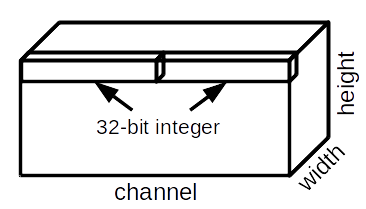
\includegraphics[width=0.5\columnwidth]{map}
\caption{Diagram of how the data is organized in the feature map of the XNOR network.}
\label{fig:map}
\end{figure}

When using XNOR networks the multiplication of two values needed when computing convolutions can be done using
\begin{equation}
\mathit{filter} \cdot \mathit{input} = 1 - 2 \cdot (\mathit{filter} \oplus \mathit{input})
\label{eq:xnor-1}
\end{equation}
where $\mathit{filter}$ is the value of the filter for a certain position and $\mathit{input}$ is the value of the input for that corresponding position. The multiplication by two in Equation (\ref{eq:xnor-1}) can in practice be implemented as a bitwise shift to the left by 1, which is a less computationally demanding operation than multiplication. Modifying Equation (\ref{eq:xnor-1}) to apply to 32-bit integers is simple and can be done using the function popcount which tells how many bits in a integer are 1.
\begin{equation}
\mathit{filter_{32}} \cdot \mathit{input_{32}} = 32 - 2 \cdot \popcount(\mathit{filter_{32}} \oplus \mathit{input_{32}})
\label{eq:xnor-32}
\end{equation}
where $\mathit{filter_{32}}$ is 32 values of the binary filter as represented in Figure \ref{fig:map} and $\mathit{input_{32}}$ is the corresponding 32 binary inputs. Therefore using Equation (\ref{eq:xnor-32}) it is possible to do 32 multiplications at the same time. On some architectures $\popcount$ is a built-in function and when that is not the case it can be implemented without using branch instructions and only using around 20 instruction cycles or less with lookup tables. Even when using floating-points with a FPU a minimum of 32 instruction cycles is required for the multiplications. In addition when multiplying values individually a loop, as well as more writes and reads to and from the memory are needed.

\subsection{Consecutive layers}
\label{sec:layers}

Another advantage of XNOR networks is that intermediary values between two binary convolutions can be manipulated without using floating-points. The intermediary layers between a binary convolution and a previous convolution layer can be simplified to three comparisons. This is because the result of the multiplication and summation of the filter with the input $x$ at one position is biased and scaled and afterwards passed through the batch normalization, ReLU and binarization layers, before going into the next binary convolution layer. All these operations can done in-line and then we would only need to store the binary output of the binarization layer. The operations performed on $x$ before the next convolutional layer can be written as
\begin{equation}
x_{\mathit{conv}} = x\cdot\alpha + \mathit{bias}
\label{eq:conv}
\end{equation}
where $\mathit{bias}$ is the bias of the filter and $\alpha$ is the scaling factor calculated based on Equation (\ref{eq:alpha}). Afterwards is the ReLU layer which is equivalent to 
\begin{equation}
x_{\mathit{ReLU}} = \max(x_{\mathit{conv}}, 0.0)
\label{eq:ReLU}
\end{equation}
The scaling and affine transform applied by the batch normalization layer from Equation (\ref{eq:bn-matrix}) is equivalent to
\begin{equation}
x_{\mathit{BatchNormalize}} = \frac{x_{\mathit{ReLU}} - \mu}{\sigma}\cdot\gamma + \beta
\label{eq:BN}
\end{equation}
And the final layer is the binarization layer which can be written using $\sign$ but it is enough to know if $x_{\mathit{BatchNormalize}}$ is greater than zero or not.
\begin{equation}
x_{\mathit{BatchNormalize}} > 0
\label{eq:binary}
\end{equation}
Now we want to know what $x$ has to be so that the condition in Equation (\ref{eq:binary}) is satisfied. We start by combining Equations (\ref{eq:BN}) and (\ref{eq:binary})
\begin{equation}
\frac{x_{\mathit{ReLU}} - \mu}{\sigma}\cdot\gamma + \beta > 0
\label{eq:x-1}
\end{equation}
Since the standard deviation $\sigma$ is by definition positive it can be moved to the right side of the inequality. The parameter $\gamma$ which is the scaling factor of the affine transform that is part of the batch normalization layer can be negative so it is only possible to divide by its absolute value. From Equation (\ref{eq:x-1}) we obtain
\begin{equation}
\sign(\gamma)\cdot x_{\mathit{ReLU}} > -\frac{\beta\sigma}{\lvert\gamma\rvert}+\sign(\gamma)\cdot\mu
\label{eq:x-2}
\end{equation}
For simplicity we denote the right side of the inequality Equation (\ref{eq:x-2}) by $M_1$ which is a floating-point constant. We continue by combining Equations (\ref{eq:x-2}), (\ref{eq:conv}) and (\ref{eq:ReLU})
\begin{equation}
\sign(\gamma)\cdot\max(x\cdot\alpha+\mathit{bias}, 0.0) > M_1
\end{equation}
From (\ref{eq:alpha}) we know that $\alpha$ is positive so we can write
\begin{equation}
\sign(\gamma)\cdot\max(x, -\frac{\mathit{bias}}{\alpha}) > \frac{M_1-sign(\gamma)\cdot\mathit{bias}}{\alpha}
\end{equation}
Again we can replace the right side of the inequality with a floating-point constant $M_2$ to obtain
\begin{equation}
\sign(\gamma)\cdot\max(x, -\frac{\mathit{bias}}{\alpha}) > M_2
\label{eq:x-3}
\end{equation}
\begin{equation}
M_2 = (-\frac{\beta\sigma}{\lvert\gamma\rvert}+\sign(\gamma)\cdot(\mu-\mathit{bias}))\cdot\frac{1}{\alpha}
\end{equation}
The constants in Equation (\ref{eq:x-3}) can be precomputed when the network is initialized which also saves memory since now we only need to store two values and a sign. In practice this can be implemented either by changing sign and doing two comparisons or by doing three comparisons and moving the sign to the right side of the inequality at initialization. When applying this simplification to the intermediary layers between two binary convolutions the added condition is that $x$ is an integer. In this case $-\frac{\mathit{bias}}{\alpha}$ and $M_2$ can be truncated to integers and we also need to store a variable that tells which one of them is larger for the special case in which they truncate to the same number but as floating-points one is greater than the other. In this way consecutive XNOR layers do not require any floating-point operations nor storing into memory any floating-point values for the XNOR layers or the layers in between them.

\subsection{Platform}
\label{sec:platform}

\begin{figure}[!t]
\centering
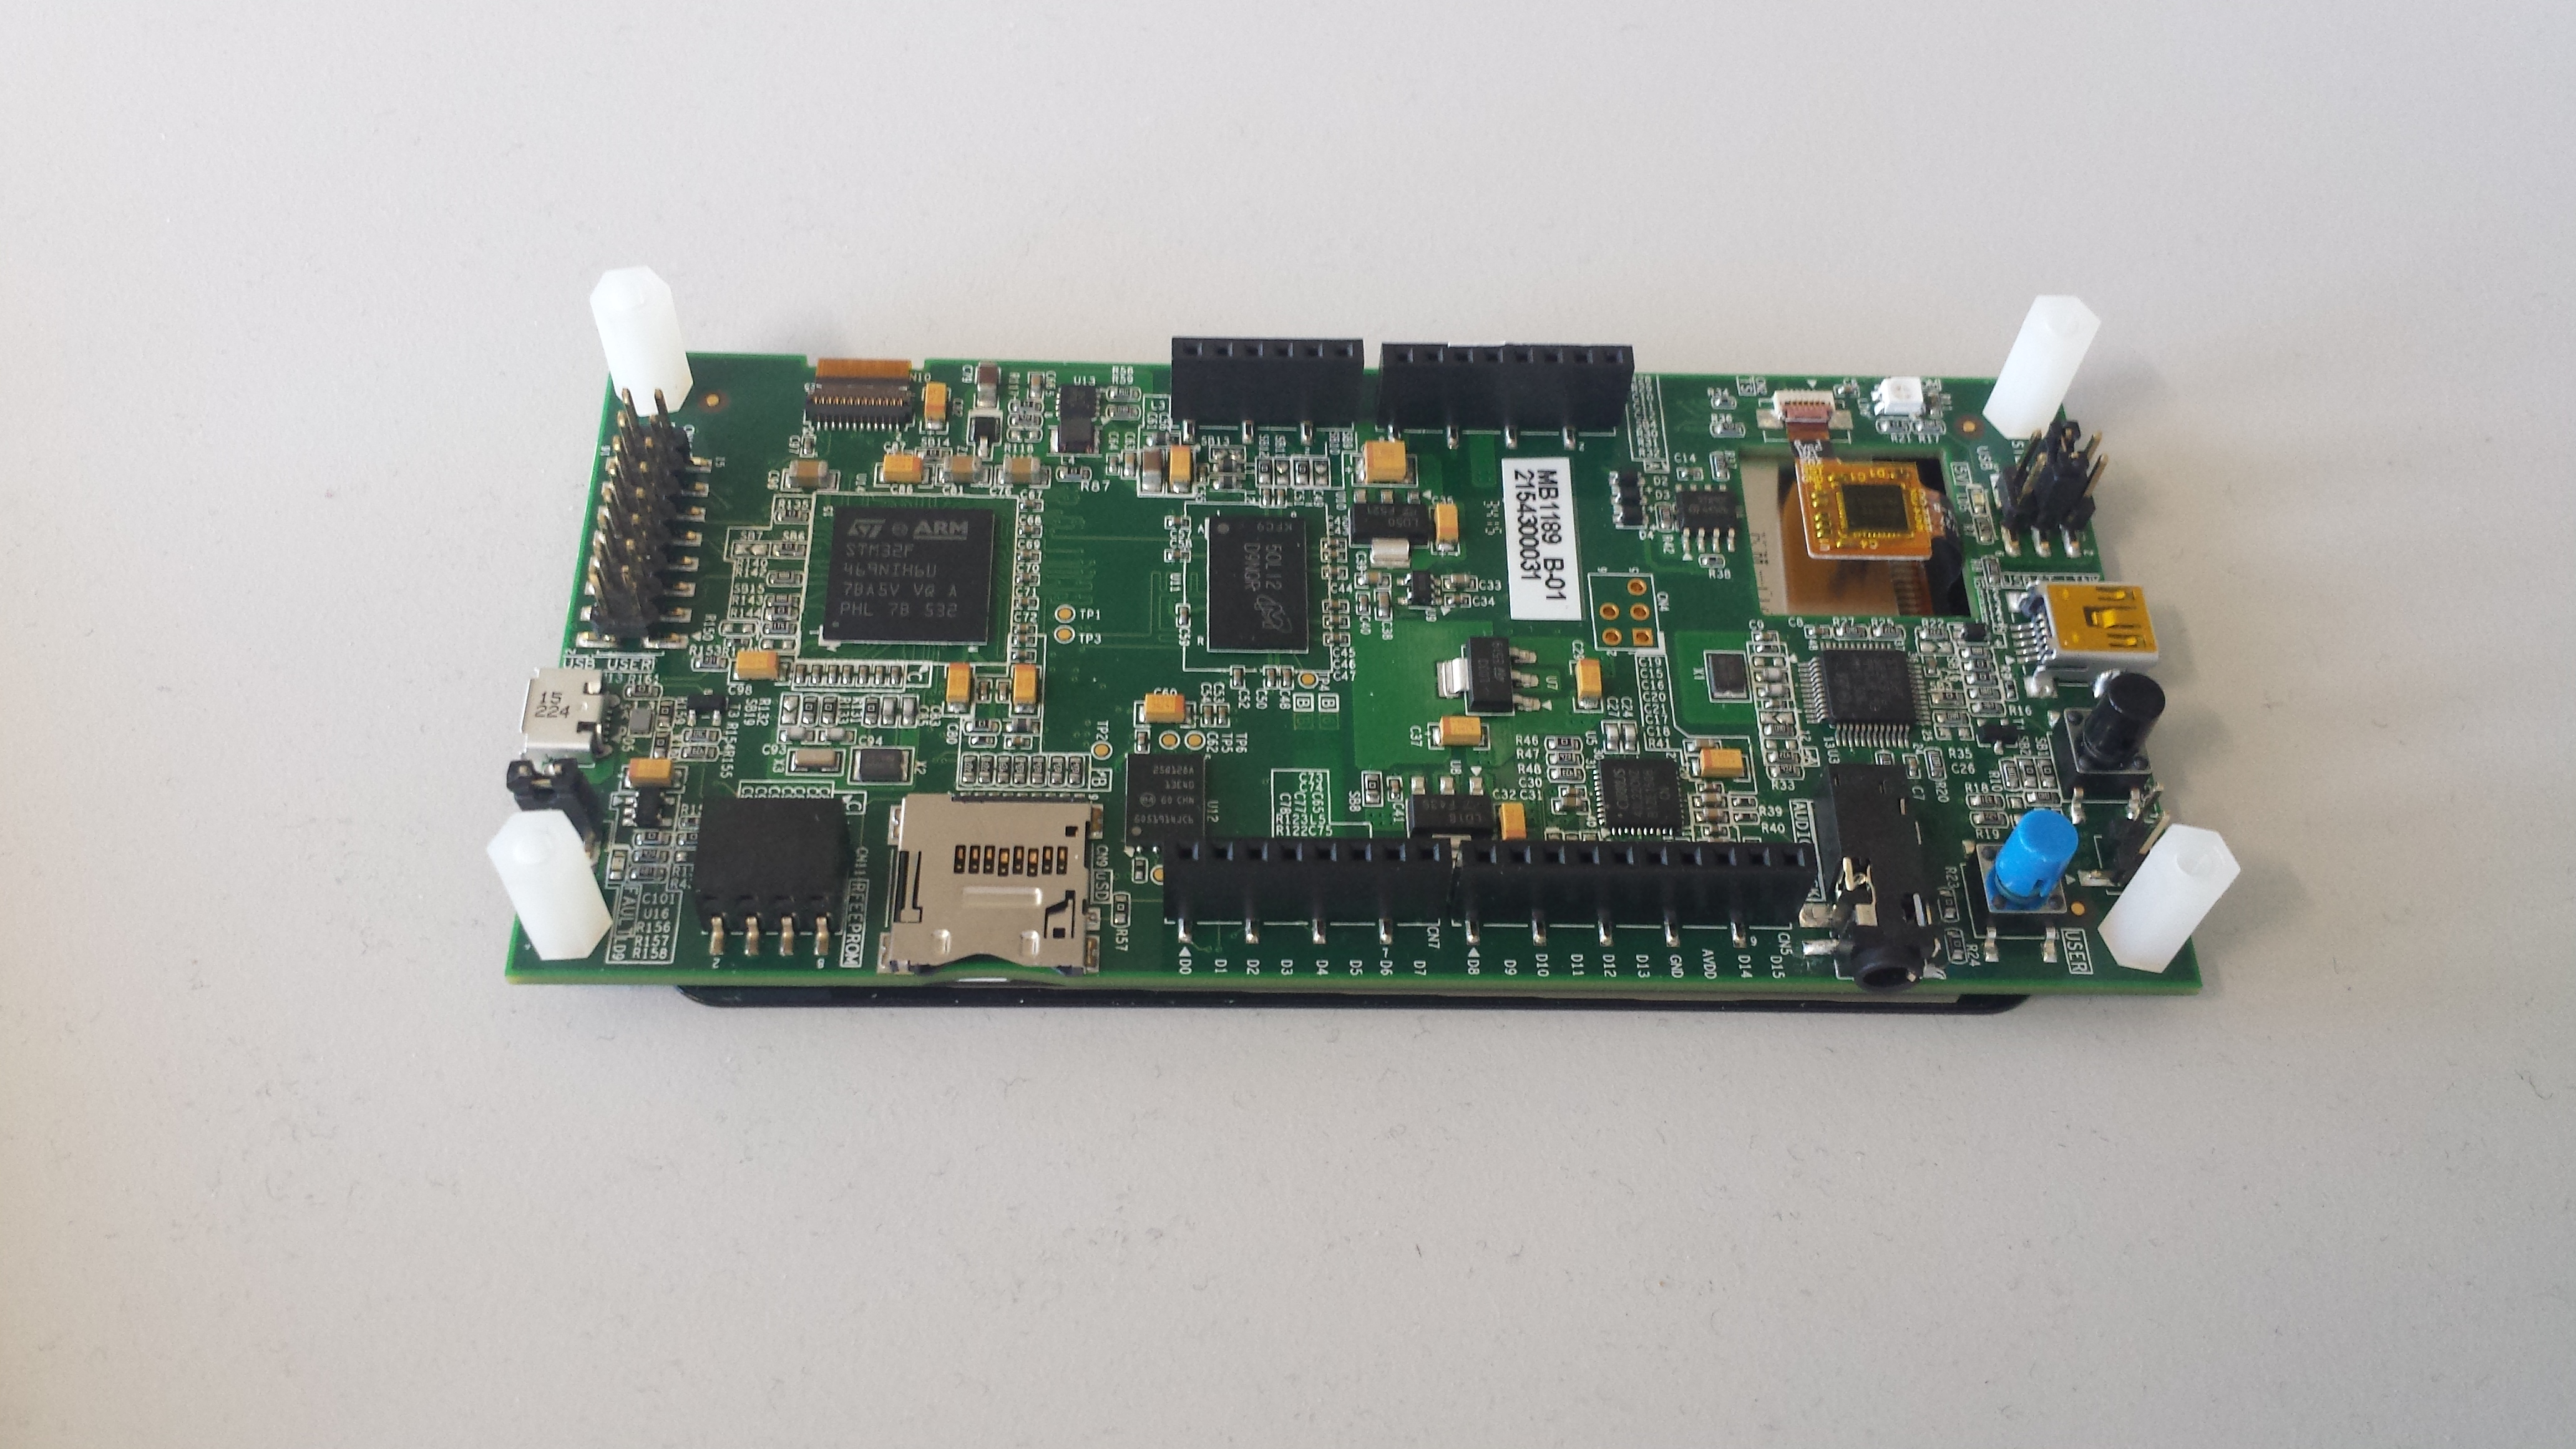
\includegraphics[width=\columnwidth]{board}
\caption{The STM32F469I Discovery board used in this project.}
\label{fig:board}
\end{figure}

\begin{table}[!t]
\renewcommand{\arraystretch}{1.3}
\caption{Characteristics of the STM32F469NI Microcontroller.}
\label{table:mcu}
\centering
\begin{tabular}{|c|c|}
\hline
Inscruction Set &  ARMv7-M (32-bit)\\
\hline
FPU & \checkmark\\
\hline
Frequency & \SI{180}{\mega\hertz}\\
\hline
SRAM & \SI{384}{\kilo\byte}\\
\hline
Flash & \SI{2}{\mega\byte}\\
\hline
Supply voltage & \SI{3.3}{\volt}\\
\hline
\end{tabular}
\end{table}

The platform on which the network was tested was a STM32F469I Discovery board from STMicroelectronics featuring an ARM M4F microcontroller. A picture of the development board is depicted in Figure \ref{fig:board}. The microcontroller has a 32-bit instruction set and contains a hardware FPU. The microcontroller has an operating voltage of \SI{3.3}{\volt} and \SI{384}{\kilo\byte} of SRAM storage. A summary of the features of the microcontroller is in Table \ref{table:mcu}. Important when doing convolutions with floating-point values is the number of cycles needed for a Multiply-Accumulate operation (MAC) which with the integrated FPU is 3. Other basic operations such as XOR, addition and subtraction only require 1 instruction cycle. Also to note is that the microcontroller does not have a built-in instruction for popcount, therefore in this case it was implemented in software.

\subsection{Memory optimizations}

The minimum amount of memory required for the XNOR network is \SI{230}{\kilo\byte} based on Tables \ref{table:feature} and \ref{table:param-xnor}. Theoretically it would be possible to run the network all at once on the microcontroller, but as a simplification the input image was divided into 4 overlapping section. This simplification allows for a more easier implementation regarding how memory buffers are allocated and used. Each overlapping section is passed separately, memorizing the result and adding all of them together at the end to obtain the final result. The overlap causes a computational overhead of 15\% and reduces the memory required for storing intermediary results to a fourth. The final implementation uses a total of \SI{190}{\kilo\byte} of memory due to overheads and theoretically simple optimizations such as buffer memory management that were not added.

Another optimization is that the last XNOR network would need to have a floating-point output for the last layer which is full-precision. To not allocate such a large floating-point buffer for only one output the last and second to last layers were combined into one. This is simply done since both convolutional layers only have $1\times 1$ filters in which case it is simple to pass the input through both of the layers at the same time. This makes separate measurements for these two layers impossible and therefore they will be referred to only as one layer in the Results section.

\section{Results}

\subsection{Training}

\begin{figure}[!t]
\centering
\subfloat[Top-1 accuracy for XNOR and full precision during the training phase]{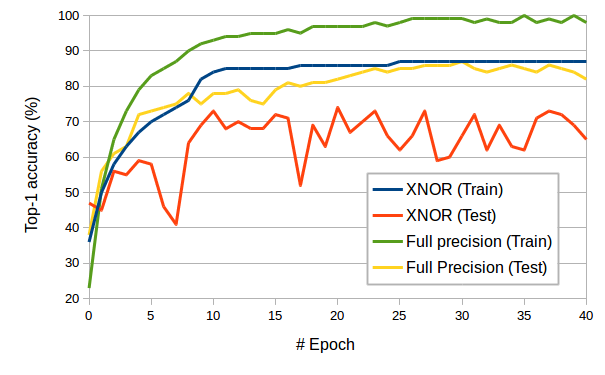
\includegraphics[width=\columnwidth]{xnor}%
\label{fig:top-1}}
\hfill
\subfloat[Top-5 accuracy for the XNOR network during the training phase]{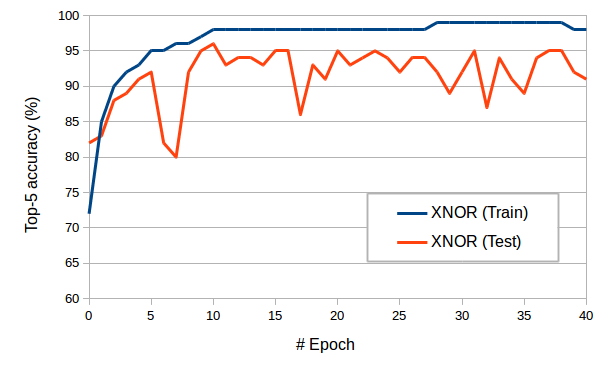
\includegraphics[width=\columnwidth]{xnor-5}%
\label{fig:top-5}}
\caption{Top-1 and top-5 accuracies during the training phase for the XNOR network also in comparison with the top-1 accuracy during training for the full precision network.}
\label{fig:accuracy}
\end{figure}

\begin{figure*}[!t]
\centering
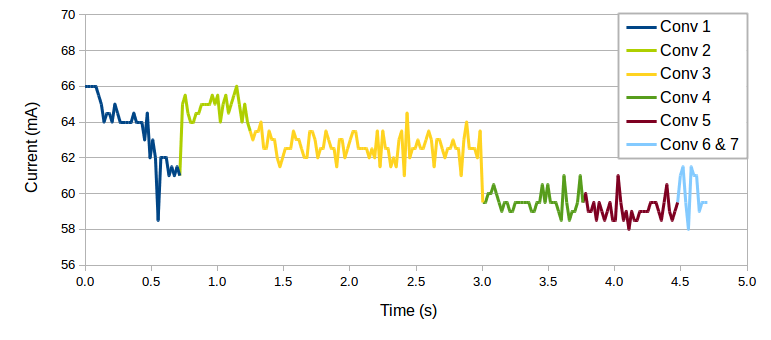
\includegraphics[width=\textwidth]{data}
\caption{Current consumption for the entire network}
\label{fig:data}
\end{figure*}

The training of the network was done using the framework Torch on a Nvidia GeForce GTX 1080 GPU with 8GB of memory. The training data was the as presented in Meyer \textit{et al.} with the same split of 75\% training data and 25\% test \cite{lukas}. The XNOR network was trained using a batch size of 64, which uses about 5GB of GPU memory and takes 2 minutes for each epoch to complete. The training was done for a total of 40 epochs. The optimizer used to train the network was Stochastic Gradient Descent (SGD), with a momentum of 0.9 and with a decaying learning rate. Starting with a learning rate of $10^{-2}$ at the beginning the XNOR network learns quickly but soon afterwards tends to overfit. To avoid this the learning rate is decrease significantly after the first 8 epochs to $10^{-4}$.

The accuracy results for the network are visible in Figure \ref{fig:accuracy}. The graph in Figure \ref{fig:top-1} compares the top-1 accuracy of the full precision network with that of the XNOR network. As can be seen the XNOR network reaches a maximum accuracy of 74\% while the full precision network reaches an accuracy of 86\% which is a difference of 12\%. The difference coincides with the results obtained by Rastegari \textit{et al.} where the binarization of the network similarly caused a 12\% drop in accuracy \cite{xnor}. The accuracy of the XNOR network on the training set remains constant but stabilizes at 88\%, which is also 12\% less than the accuracy, on the training set, of the full precision network which stabilizes at 100\%. As seen in Figure \ref{fig:top-5}, the top-5 accuracy reached by the full precision network is 100\% while the XNOR network only manages to reach 95\% on the test set.

The classification accuracy of the XNOR network on the test set in Figure \ref{fig:top-1} is stable on average but has a large variance compared to the full precision network. This instability is because of the binarization of the weights as well as the activations which causes the XNOR network to have trouble fully representing the internal structure of the data. This also makes the XNOR network very sensitive to changes, for example removing the ReLU layers causes an almost 20\% drop in accuracy. Similarly for example removing the first batch normalization layer reduces the average accuracy by 5\%. As mentioned in Section \ref{sec:net} the first and last layers are not binarized since this brings only a small benefit causes a significant drop in accuracy. Binarizing the weights and activations for the last layer causes a 10\% drop in accuracy and similarly binarizing the first layers weight and activations causes a complete loss in accuracy.

\subsection{Forward pass}

\begin{table}[!t]
\renewcommand{\arraystretch}{1.3}
\caption{Time necessary to compute each convolutional layer in the XNOR network for the whole input image.}
\label{table:time}
\centering
\begin{tabular}{|c|c|c|}
\multicolumn{1}{c}{\bfseries Conv layer} & \multicolumn{1}{c}{\bfseries Time (\SI{}{\second})} & \multicolumn{1}{c}{\bfseries Energy (\SI{}{\joule})} \\
\hline
1 & \SI{3.2}{} & \SI{0.67}{}\\
\hline
2 & \SI{2.0}{} & \SI{0.42}{}\\
\hline
3 & \SI{6.4}{} & \SI{1.31}{}\\
\hline
4 & \SI{3.0}{} & \SI{0.60}{}\\
\hline
5 & \SI{3.0}{} & \SI{0.60}{}\\
\hline
6 \& 7 & \SI{1.2}{} & \SI{0.24}{}\\
\hline
\multicolumn{1}{c}{\bfseries Total} & \multicolumn{1}{c}{\bfseries \SI{19}{\second}} & \multicolumn{1}{c}{\bfseries \SI{3.8}{\joule}}\\
\end{tabular}
\end{table}

\begin{table}[!t]
\renewcommand{\arraystretch}{1.3}
\caption{Total number of MACs necessary for the full image for each layer of the full precision network taken based on Meyer \textit{et al.} \cite{lukas}.}
\label{table:mac}
\centering
\begin{tabular}{|c|c|c|c|}
\multicolumn{1}{c}{\multirow{2}{*}{\bfseries Conv layer}} & \multicolumn{1}{c}{\bfseries \multirow{2}{*}{MACs}} & \multicolumn{1}{c}{\bfseries Throughput} &  \multicolumn{1}{c}{\bfseries Efficiency}\\
\multicolumn{1}{c}{\quad} & \multicolumn{1}{c}{\quad} & \multicolumn{1}{c}{\bfseries (\SI{}{MAC\per\second})} &  \multicolumn{1}{c}{\bfseries (\SI{}{MAC\per J})}\\
\hline
1 & \SI{7.4}{M} & \SI{2.3}{M} & \SI{11}{M}\\
\hline
2 & \SI{118}{M} & \SI{59}{M} & \SI{281}{M}\\
\hline
3 & \SI{472}{M} & \SI{74}{M} & \SI{360}{M}\\
\hline
4 & \SI{236}{M} & \SI{79}{M} & \SI{393}{M}\\
\hline
5 & \SI{236}{M} & \SI{79}{M} & \SI{393}{M}\\
\hline
6 \& 7 & \SI{32}{M} & \SI{27}{M} & \SI{133}{M}\\
\hline
\multicolumn{1}{c}{\bfseries Total/Average} & \multicolumn{1}{c}{\bfseries \SI{1100}{M}} & \multicolumn{1}{c}{\bfseries \SI{58}{M}}& \multicolumn{1}{c}{\bfseries \SI{290}{M}}\\
\end{tabular}
\end{table}

The algorithm was tested on the development board described in Section \ref{sec:platform} and the current consumed by the microcontroller was measured using a Keysight N6705A power analyzer. The resulting current for each layer was differentiated using a trigger signal. The graph for the current usage of the microcontroller can be seen in Figure \ref{fig:data}. Figure \ref{fig:data} only represents passing one fourth of the input through the network, for a full prediction four such cycles are required. Since the microcontroller operates at a voltage of \SI{3.3}{\volt} and the time it takes to compute each layer is know from Table \ref{table:time} it is possible to calculate the required energy for each layer. Classifying 2.5 seconds of audio therefore takes 19 seconds and requires \SI{3.8}{\joule} energy.

The efficiency and throughput of the network can be calculated using Table \ref{table:time} and the number of MACs for each convolutional layer calculated by Meyer \textit{et al} \cite{lukas}. The results are shown in Table \ref{table:mac} from where we can see that the total throughput for the XNOR network is \SI{58}{M MAC\per\second} and the energy efficiency is \SI{290}{M MAC\per\joule}. Of interest are also the throughputs for the full precision and XNOR convolutional layers. We will ignore the last row which contains the last two layers of the network combined together since one is a XNOR layer and the other is full precision. We can estimate the throughput and efficiency of a full precision layer to be equal to that of the first layer. Averaging the throughputs of the layers 2 to 5 we get an average throughput of \SI{74}{M MAC\per\second} and an average efficiency of \SI{370}{M MAC\per\joule}. Since it is not possible to test the network using full precision layers on the microcontroller we can use the previously calculated values to extrapolate that the full precision network would require 8 minutes and 100J of energy. Which is 25 times slower than the XNOR network and in consequence also consumes 26 times more energy.

\section{Conclusions}

\begin{table}[!t]
\renewcommand{\arraystretch}{1.3}
\caption{Comparison between a XNOR and a full precision network. Values marked with a ($^*$) were extrapolated from existing measurements.}
\label{table:compare}
\centering
\begin{tabular}{|c|c|c|}
\multicolumn{1}{c}{\quad} & \multicolumn{1}{c}{\bfseries XNOR} &  \multicolumn{1}{c}{\bfseries Full precision}\\
\cline{2-3}
\multicolumn{1}{c|}{\bfseries Memory} & \SI{230}{\kilo\byte} & \SI{6380}{\kilo\byte}\\
\cline{2-3}
\multicolumn{1}{c|}{\bfseries Accuracy (top-1)} & 74\% & 86\%\\
\cline{2-3}
\multicolumn{1}{c|}{\bfseries Accuracy (top-5)} & 96\% & 100\%\\
\cline{2-3}
\multicolumn{1}{c|}{\bfseries MACs} & \SI{1100}{M} & \SI{1100}{M}\\
\cline{2-3}
\multicolumn{1}{c|}{\bfseries Time} & \SI{19}{\second} & \SI{480}{\second}$^*$\\
\cline{2-3}
\multicolumn{1}{c|}{\bfseries Energy} & \SI{3.8}{\joule} & \SI{100}{\joule}$^*$\\
\cline{2-3}
\multicolumn{1}{c|}{\bfseries Throughput} & \SI{58}{M MAC\per\second} & \SI{2.3}{M MAC\per\second}$^*$\\
\cline{2-3}
\multicolumn{1}{c|}{\bfseries Efficincy} & \SI{290}{M MAC\per\joule} & \SI{11}{M MAC\per\joule}$^*$\\
\cline{2-3}
\end{tabular}
\end{table}

A final overview of the differences between a XNOR and a full precision network is in Table \ref{table:compare}. The XNOR network proved to be more efficient than the full precision network, using 28 times less memory and being 25 times faster and 26 times more energy efficient. On the other hand the XNOR network suffers a loss in precision of 12\% when compared to the original network which is consistent with the results obtained also in \cite{xnor} for another network. When comparing top-5 accuracies the loss is not as significant as the XNOR network has a 96\% top-5 accuracy and the full-precision network has a 100\% top-5 accuracy. The input image was split into 4 smaller images to simplify the forward pass. This caused the algorithm to be 15\% slower than what was theoretically possible but allowed for simplifications regarding the memory management. Therefore the network could be optimized further.

What was seen during training is that even small changes to the structure of the XNOR network had large effects in the accuracy and how easily the network would over-learn. Also the optimizer and its parameters had a very large effect on the outcome of the training. The fact that the accuracy on the training set never reached 100\% in combination with the previous observations open the possibility that it could be possible to recoup the loss in accuracy through changes to the network structure and training process. The structure presented in this project is one of many structures that seemed to be the most stable and accurate and there is place for further improvement and the possibility of recouping the loss in accuracy.

The final implementation only used a total of \SI{190}{kB} memory, which can still be significantly reduced. The use of a FPU was limited to only the first and last layer as well as the initialization of the network. This initialization can be done beforehand and the parameters described in Section \ref{sec:layers} can be passed directly to the network. The XNOR network did not completely eliminate the need for floating-point operations, but it reduced the amount to only 1\% of the total number of operations. With the reduced amount of floating-point operations needed the XNOR network can also run on a microcontroller that does not have a FPU but uses fixed-point operations.

As a conclusion running simplified version of full precision CNNs on microcontroller and small embedded systems is possible if a loss in accuracy of around 10\% is acceptable. In some applications this can be acceptable, for example outdoor sensors or satellites where the cost of transmitting the raw data would be more costly than processing the data locally and only transmitting the result. Using CNNs on embedded platforms would also be useful for cases in which transmitting the data is not desirable for example due to privacy concerns. There exist also systems that can not transmit or need to be able to operate also in cases when transmission fails, such as autonomous robots or self driving cars.

% An example of a floating figure using the graphicx package.
% Note that \label must occur AFTER (or within) \caption.
% For figures, \caption should occur after the \includegraphics.
% Note that IEEEtran v1.7 and later has special internal code that
% is designed to preserve the operation of \label within \caption
% even when the captionsoff option is in effect. However, because
% of issues like this, it may be the safest practice to put all your
% \label just after \caption rather than within \caption{}.
%
% Reminder: the "draftcls" or "draftclsnofoot", not "draft", class
% option should be used if it is desired that the figures are to be
% displayed while in draft mode.
%
%\begin{figure}[!t]
%\centering
%\includegraphics[width=2.5in]{myfigure}
% where an .eps filename suffix will be assumed under latex, 
% and a .pdf suffix will be assumed for pdflatex; or what has been declared
% via \DeclareGraphicsExtensions.
%\caption{Simulation results for the network.}
%\label{fig_sim}
%\end{figure}

% Note that the IEEE typically puts floats only at the top, even when this
% results in a large percentage of a column being occupied by floats.


% An example of a double column floating figure using two subfigures.
% (The subfig.sty package must be loaded for this to work.)
% The subfigure \label commands are set within each subfloat command,
% and the \label for the overall figure must come after \caption.
% \hfil is used as a separator to get equal spacing.
% Watch out that the combined width of all the subfigures on a 
% line do not exceed the text width or a line break will occur.
%
%\begin{figure*}[!t]
%\centering
%\subfloat[Case I]{\includegraphics[width=2.5in]{box}%
%\label{fig_first_case}}
%\hfil
%\subfloat[Case II]{\includegraphics[width=2.5in]{box}%
%\label{fig_second_case}}
%\caption{Simulation results for the network.}
%\label{fig_sim}
%\end{figure*}
%
% Note that often IEEE papers with subfigures do not employ subfigure
% captions (using the optional argument to \subfloat[]), but instead will
% reference/describe all of them (a), (b), etc., within the main caption.
% Be aware that for subfig.sty to generate the (a), (b), etc., subfigure
% labels, the optional argument to \subfloat must be present. If a
% subcaption is not desired, just leave its contents blank,
% e.g., \subfloat[].


% An example of a floating table. Note that, for IEEE style tables, the
% \caption command should come BEFORE the table and, given that table
% captions serve much like titles, are usually capitalized except for words
% such as a, an, and, as, at, but, by, for, in, nor, of, on, or, the, to
% and up, which are usually not capitalized unless they are the first or
% last word of the caption. Table text will default to \footnotesize as
% the IEEE normally uses this smaller font for tables.
% The \label must come after \caption as always.
%
%\begin{table}[!t]
%% increase table row spacing, adjust to taste
%\renewcommand{\arraystretch}{1.3}
% if using array.sty, it might be a good idea to tweak the value of
% \extrarowheight as needed to properly center the text within the cells
%\caption{An Example of a Table}
%\label{table_example}
%\centering
%% Some packages, such as MDW tools, offer better commands for making tables
%% than the plain LaTeX2e tabular which is used here.
%\begin{tabular}{|c||c|}
%\hline
%One & Two\\
%\hline
%Three & Four\\
%\hline
%\end{tabular}
%\end{table}


% Note that the IEEE does not put floats in the very first column
% - or typically anywhere on the first page for that matter. Also,
% in-text middle ("here") positioning is typically not used, but it
% is allowed and encouraged for Computer Society conferences (but
% not Computer Society journals). Most IEEE journals/conferences use
% top floats exclusively. 
% Note that, LaTeX2e, unlike IEEE journals/conferences, places
% footnotes above bottom floats. This can be corrected via the
% \fnbelowfloat command of the stfloats package.



% trigger a \newpage just before the given reference
% number - used to balance the columns on the last page
% adjust value as needed - may need to be readjusted if
% the document is modified later
%\IEEEtriggeratref{8}
% The "triggered" command can be changed if desired:
%\IEEEtriggercmd{\enlargethispage{-5in}}

% references section

% can use a bibliography generated by BibTeX as a .bbl file
% BibTeX documentation can be easily obtained at:
% http://mirror.ctan.org/biblio/bibtex/contrib/doc/
% The IEEEtran BibTeX style support page is at:
% http://www.michaelshell.org/tex/ieeetran/bibtex/
%\bibliographystyle{IEEEtran}
% argument is your BibTeX string definitions and bibliography database(s)
%\bibliography{IEEEabrv,../bib/paper}
%
% <OR> manually copy in the resultant .bbl file
% set second argument of \begin to the number of references
% (used to reserve space for the reference number labels box)
\begin{thebibliography}{99}

\bibitem{best1}
A. Krizhevsky, I. Sutskever, and G. Hinton. ImageNet classification with deep convolutional neural networks. NIPS, 2012.

\bibitem{best2}
S.C. Turaga, J.F. Murray, V. Jain \textit{et al.}. Convolutional networks can learn to generate affinity graphs for image segmentation. Neural Computation, 2010.

\bibitem{best3}
G. Hinton, L. Deng, G. E. Dahl \textit{et al}. Deep neural networks for acoustic modeling in speech recognition. IEEE Signal Processing Magazine, Nov. 2012.

\bibitem{iot}
F. Xia, L.T. Yang, L. Wang \textit{et al.}. Internet of Things. International Journal of Communication Systems, 2012

\bibitem{robots}
Y. LeCun, K. Kavukcuoglu, C. Farabet. Convolutional Networks and Applications in Vision. ISCAS, 2010

\bibitem{alexnet}
A. Krizhevsky, I. Sutskever, G.E. Hinton. ImageNet Classification with Deep Convolutional
Neural Networks. Advances in neural information processing systems, NIPS, 2012 

\bibitem{deep}
J. Ba R. Caruana. Do Deep Nets Really Need to be Deep?. Advances in Neural Information Processing Systems 27, NIPS, 2014.

\bibitem{compact1}
C. Szegedy, W. Liu, Y. Jia \textit{et al.}. Going Deeper with Convolutions. Proceedings of the IEEE Conference on Computer Vision and Pattern Recognition, 2015.

\bibitem{compact2}
C. Szegedy, S. Ioffe, V. Vanhoucke. Inception-v4, Inception-ResNet and the Impact of Residual Connections on Learning. arXiv preprint arXiv:1602.07261, 2016.

\bibitem{prune}
S. Han, J. Pool, J. Tran, W. Dally. Learning both weights and connections for efficient neural network. Advances in Neural Information Processing Systems 28, NIPS, 2015.

\bibitem{quantize}
S. Han, H. Mao, W.J. Dally. Deep compression: Compressing deep neural network with pruning, trained quantization and huffman coding. ICLR, 2016.

\bibitem{binary}
M. Courbariaux, I. Hubara, D. Soudry \textit{et al.}. Binarized Neural Networks: Training Neural Networks with Weights and Activations Constrained to +1 or -1. arXiv preprint arXiv:1602.02830v3, March 2016.

\bibitem{xnor}
M. Rastegari, V. Ordonez, J. Redmon \textit{et al.}. XNOR-Net: ImageNet Classification Using Binary Convolutional Neural Networks. arXiv preprint arXiv:1603.05279v4, Aug 2016

\bibitem{lukas}
M. Meyer, L. Cavigelli, L. Thiele. Efficient convolutional neural network for audio event detection. ICASSP, 2017

\bibitem{imagenet}
ImageNet 2012 dataset \url{http://www.image-net.org/challenges/LSVRC/2012/}

\bibitem{imagenet-res}
Results for ImageNet 2016 \url{http://image-net.org/challenges/LSVRC/2016/results}

\bibitem{mfcc}
B. Logan. Mel Frequency Cepstral Coefficients for Music Modeling. ISMIR, 2000

\end{thebibliography}




% that's all folks
\end{document}


